\documentclass[11pt,a4paper]{article}
\usepackage[margin=2.3cm]{geometry}
\usepackage[T1]{fontenc}
\usepackage{lmodern}
\usepackage{microtype}
\usepackage{amsmath}
\usepackage{booktabs}
\usepackage{tabularx}
\usepackage{graphicx}
\usepackage{enumitem}
\usepackage{caption}
\usepackage{float}
\usepackage[hidelinks]{hyperref}
\setlist{itemsep=2pt,topsep=4pt}
\captionsetup{font=small,labelfont=bf}
\newcommand{\code}[1]{\texttt{#1}}
\newcommand{\pt}{\,pts}
\newenvironment{stepbox}[1]{\par\medskip\noindent\textbf{#1}\par\nopagebreak}{\par}

\title{\textbf{Emoji Vendor Classification}\\[3pt]
\large A step-by-step account of the strategy, the experiments and the decisions}
\author{Erdem Sanver\\\small Computer Vision 2026 -- BSc AIDAMS -- Final Project (team \emph{The Winners})}
\date{18 October 2026}

\begin{document}
\maketitle

\begin{abstract}
\noindent This document explains, in the order in which it happened, everything I did for the Kaggle
challenge: how the evaluation protocol was set up, what the data analysis revealed, each experiment
(also the ones that were never submitted or that failed), why it was run, how exactly it was
configured, what came out and which decision followed. The team's public score went from 0.788 to
0.981 public and 0.98238 private (E15, the team's best entry; 5th of 18 teams on the final private leaderboard). Every experiment is also logged, with the same
information in short form, in \code{results/Strategies Computer Vision Project.xlsx}.
\end{abstract}

\tableofcontents
\bigskip

%=====================================================================
\section{Starting point and overall strategy}

\paragraph{The task.} Each image shows one emoji; the label is the vendor whose design it is:
apple, google, whatsapp, facebook, samsung, mozilla or messenger. The same emoji (e.g.\ a bucket)
exists in several vendor styles, so the model must learn \emph{how} something is drawn, not
\emph{what} is drawn. There are 9\,879 labelled training images and 9\,879 unlabelled test images;
the metric is accuracy. The public leaderboard uses about half of the test set, the final
(private) ranking the other half.

\paragraph{Where the team stood.} Before this work the team had four submissions, all from a
small CNN trained from scratch on 96\,px RGB images: 0.775, 0.788 and 0.783 (one more scored 0.000
because of an output-format mistake). The leaderboard top was 0.998, then 0.987 and 0.984.

\paragraph{Constraints that shaped the strategy.}
\begin{itemize}[leftmargin=*]
\item \emph{Time:} six days to the deadline.
\item \emph{Submissions:} 5 per day, shared by the whole team. Using Kaggle to evaluate every idea was
therefore not an option.
\item \emph{Compute:} a laptop (Apple M4, 16\,GB, PyTorch with the MPS GPU backend). A 224\,px
ConvNeXt run takes 1.5--2 hours, so experiments had to be chosen carefully.
\item \emph{Grading:} the grade also depends on a written report, every student must be able to
explain every part of the solution, and the work must be reproducible.
\end{itemize}

\paragraph{The strategy.} From these constraints I derived four working rules:
\begin{enumerate}[leftmargin=*]
\item \textbf{Decide on a local validation set, not on the leaderboard.} A fixed stratified 80/20
split of the training data (seed 42) gives 7\,903 training and 1\,976 validation images with the same
class proportions. Kaggle is used only to confirm models that are already good locally.
\item \textbf{Change one variable at a time.} Each experiment differs from a reference run in one
aspect only (preprocessing, architecture, resolution, \dots), so the effect can be attributed.
\item \textbf{Climb a ladder from simple to complex}: metadata-only diagnostic $\to$ classical
features $\to$ CNN from scratch $\to$ transfer learning $\to$ stronger architecture $\to$ resolution
$\to$ ensembles $\to$ more data. Each rung tells the report something.
\item \textbf{Log everything automatically.} Each run writes a JSON record (configuration, scores,
per-class confusion matrix, training curve, runtime); the Excel sheet requested by the course is
regenerated from these records, so no number is typed by hand.
\end{enumerate}

\paragraph{How reliable is a validation difference?} With 1\,976 validation images and accuracy
around 0.97, one standard error is $\sqrt{0.97\cdot0.03/1976}\approx0.4$ points; at 0.94 it is about
0.5 points. I therefore treat differences below about 0.3--0.4 points (8 images or fewer) as noise.

%=====================================================================
\section{Step 1 -- Understanding the data}

\begin{stepbox}{What I looked at}
Label distribution, image sizes, PNG colour modes and transparency, for every training and test image.
\end{stepbox}

\paragraph{Class imbalance.} apple 1\,924, google 1\,877, samsung 1\,790, facebook 1\,667,
whatsapp 1\,644, messenger 580, mozilla 397. Mozilla is only 4\% of the data. Because accuracy
favours the large classes, I additionally track \emph{macro} precision (the average over classes),
which weights mozilla as much as apple.

\paragraph{Heterogeneous files.} The PNGs come in five colour modes (RGBA, P = palette, LA, RGB, L)
and mainly three sizes. Cross-tabulating size and label showed that the size almost determines the
vendor:

\begin{table}[H]
\centering\small
\begin{tabular}{lrrrrl}
\toprule
 & 72\,px & 160\,px & 240\,px & other & dominant PNG mode \\
\midrule
apple     & 1\,922 & 2 & -- & -- & RGBA \\
samsung   & 1\,784 & -- & -- & 6 & P (palette), 1\,580 of 1\,790 \\
google    & 1\,756 & -- & 3 & 118 & RGBA (116 are 72$\times$68) \\
whatsapp  & 147 & 1\,484 & -- & 13 & RGBA \\
facebook  & 117 & -- & 1\,550 & -- & RGBA \\
messenger & 8 & -- & 572 & -- & RGBA \\
mozilla   & 35 & -- & 362 & -- & RGBA \\
\bottomrule
\end{tabular}
\caption{Source image size and colour mode per vendor (training set). The test set has the same distribution.}
\end{table}

\paragraph{Hidden colours under transparency.} About 43\% of the pixels of a typical image are fully
transparent. In a PNG, a transparent pixel still stores an RGB value, and that value is
vendor-specific: black for most vendors, $(76,105,113)$ for 1\,427 Samsung images, $(71,112,76)$ for
some Samsung and Apple images. The usual loading code \code{Image.open(f).convert("RGB")} simply drops
the alpha channel, so this hidden colour becomes the visible background of the emoji.

\begin{stepbox}{Experiment E1a -- how strong is this shortcut?}
\emph{Setup:} random forest (300 trees) trained on 10 numbers per image that contain \emph{no
pixel content}: width, height, one-hot PNG mode, and the RGB value under the first transparent pixel.\\
\emph{Result:} \textbf{0.658} validation accuracy (macro precision 0.631). For comparison, random
guessing gives 0.14 and always answering ``apple'' gives 0.195.
\end{stepbox}

\paragraph{Decision.} A model can obtain a large part of the score without ever looking at the
emoji. That is not computer vision, and it would also make comparisons between methods
misleading (a method could look good because it exploits the shortcut better). From here on every
model receives a \textbf{normalised image}: the RGBA image is alpha-composited onto a white
background (exactly what a person sees on a white page) and resized to a fixed square size. This
removes the hidden colour and the size information. (Later, in Step 11, I checked that this costs
nothing in accuracy.)

%=====================================================================
\section{Step 2 -- A classical computer-vision baseline (E1b)}

\begin{stepbox}{Why}
Before training neural networks I wanted a reference point that uses hand-crafted features, as in
the first part of the course, to see how far ``colour + edges'' get us.
\end{stepbox}

\paragraph{Setup.} Images composited on white and resized to 64$\times$64. Two feature groups are
concatenated (2\,276 dimensions): (i) a colour histogram with 8 bins per RGB channel
($8^3=512$ bins), normalised to sum to 1, which captures the palette; (ii) HOG on the grayscale
image (9 orientations, 8$\times$8 pixel cells, 2$\times$2 blocks), which captures edge orientation and
outline structure. Features are standardised and fed to an RBF-kernel SVM ($C=10$).

\paragraph{Result.} \textbf{0.813} validation accuracy, macro precision 0.848, training accuracy
1.000. This already beats the team's CNN on Kaggle (0.788).

\paragraph{Interpretation.} Colour palette and edge statistics carry a lot of vendor style. But the
SVM separates the training set perfectly while losing 19 points on validation: the 2\,276
fixed features are not expressive enough to capture finer cues such as shading, gradients and line
thickness, and the classifier compensates by memorising. Learned features are the next step.

%=====================================================================
\section{Step 3 -- CNN from scratch and the preprocessing ablation (E2, E3)}

\paragraph{Architecture.} A deliberately small CNN, similar to the team's earlier model, so that the
effect of preprocessing can be measured on a familiar setup: three blocks of
[conv 3$\times$3 -- BatchNorm -- ReLU] $\times$2 + max-pooling with 32, 64 and 128 channels, global
average pooling, dropout 0.3 and a linear layer: 288\,359 parameters.

\paragraph{Training (shared by all neural networks unless stated).} Cross-entropy loss; AdamW
(weight decay $10^{-4}$); one-cycle learning-rate schedule (15\% warm-up, then cosine decay);
inputs scaled to $[0,1]$ and normalised with the ImageNet mean/std; batch size 64; seed 42. For this
small CNN: learning rate $10^{-3}$, 15 epochs, 96$\times$96 input.

\begin{stepbox}{E2 vs E3 -- only the preprocessing differs}
E2: default \code{convert("RGB")} (hidden colours visible). E3: alpha-composited on white.
\end{stepbox}

\begin{table}[H]
\centering\small
\begin{tabular}{lcccccccc}
\toprule
 & acc & macro prec & apple & google & whatsapp & facebook & mozilla & messenger \\
\midrule
E2 naive RGB & 0.921 & 0.907 & 0.932 & 0.963 & 0.866 & 0.886 & 0.848 & 0.845 \\
E3 white bg  & \textbf{0.936} & \textbf{0.928} & 0.953 & 0.976 & 0.900 & 0.925 & 0.835 & 0.879 \\
\bottomrule
\end{tabular}
\caption{Validation accuracy, macro precision and per-class recall (samsung omitted: 0.989 / 0.961).}
\end{table}

\paragraph{Interpretation.} Correct alpha handling gives $+1.5$\pt{} accuracy and $+2.2$\pt{} macro
precision, even though it \emph{removes} information that is correlated with the label. The network
now sees clean shapes on a uniform canvas, which helps most for whatsapp, facebook and messenger.
Samsung recall drops (0.989$\to$0.961): with the naive conversion the model was partly recognising
Samsung by its grey-green background, which confirms the shortcut of Step~1.

\paragraph{First submission: checking the format and the protocol.} The overview page shows a
submission example with digits, while \code{train\_labels.csv} contains vendor names. Since a
format error gives 0.000 (as happened to a teammate), the first submission (E3) served to settle
this: labels written as vendor names scored \textbf{0.93642} public, against 0.9362 on our
validation split. This confirmed both the format and, more importantly, that \textbf{our validation
split predicts the leaderboard}, which justified the whole local-validation strategy. On all later
submissions the gap stayed below 0.3 points.

\paragraph{Observation on the training curve.} The validation accuracy of E3 oscillates strongly in
the first 9 epochs (e.g.\ 0.81 $\to$ 0.62 $\to$ 0.72) before converging (Figure~\ref{fig:curves}). This
is typical of the high-learning-rate phase of the one-cycle schedule combined with BatchNorm
statistics that are still moving; it settles once the learning rate decays.

%=====================================================================
\section{Step 4 -- Transfer learning: frozen vs fine-tuned (E4, E5)}

\paragraph{Motivation.} Pretrained ImageNet networks are the standard way to get strong features
from little data. The question for the report: is it enough to reuse those features, or must the
network be adapted?

\begin{stepbox}{E4 -- feature extraction}
ResNet18 with ImageNet weights, input 128$\times$128 (white background). All convolutional layers are
frozen, BatchNorm layers kept in evaluation mode, only the final linear layer is trained (3\,591 of
11.2\,M parameters). Learning rate $3\cdot10^{-3}$, 10 epochs.
\end{stepbox}
\noindent\emph{Result:} \textbf{0.775} -- worse than the SVM (0.813) and much worse than the small CNN
from scratch (0.936). Mozilla recall is only 0.57.

\begin{stepbox}{E5 -- full fine-tuning}
Same network and input, but all 11.2\,M parameters are updated (learning rate $5\cdot10^{-4}$, 10 epochs).
\end{stepbox}
\noindent\emph{Result:} \textbf{0.937} ($+16.2$\pt{} over E4), training accuracy 1.000.

\paragraph{Interpretation.} ImageNet features are built to tell \emph{objects} apart (dog vs car). Here
all classes contain the same objects; what differs is rendering style: outline thickness,
gradients, highlights, proportions. Frozen generic features do not encode these differences well,
so the linear head cannot separate the vendors. Once the whole network is allowed to adapt, the
pretrained weights become a good starting point: E5 reaches the from-scratch CNN's accuracy after
only 3--4 epochs, and its strongest gains are on messenger (0.879$\to$0.940). But it also memorises the
training set completely (training loss 0.008), which pointed to overfitting as the next problem.

%=====================================================================
\section{Step 5 -- Choosing the architecture (E5, E6, E6b)}

All three runs use full fine-tuning, the same 128\,px white-background input and 10 epochs; only the
backbone changes.

\begin{table}[H]
\centering\small
\begin{tabular}{lrrcccc}
\toprule
Backbone & params & time & val acc & macro prec & whatsapp & facebook / mozilla \\
\midrule
ResNet18 (E5)        & 11.2\,M & 5 min  & 0.937 & 0.938 & 0.891 & 0.919 / 0.848 \\
EfficientNet-B0 (E6) & 4.0\,M  & 10 min & 0.931 & 0.929 & 0.891 & 0.886 / 0.835 \\
ConvNeXt-Tiny (E6b)  & 27.8\,M & 19 min & \textbf{0.959} & \textbf{0.961} & 0.936 & 0.910 / 0.949 \\
\bottomrule
\end{tabular}
\caption{Architecture comparison (learning rates: $5\cdot10^{-4}$, $10^{-3}$, $2\cdot10^{-4}$; ConvNeXt batch 32).}
\end{table}

\paragraph{Interpretation.} EfficientNet-B0 brings no advantage at 128\,px (its compound scaling was
designed around 224\,px) and is twice as slow on the Mac because depthwise convolutions are poorly
optimised on MPS. ConvNeXt-Tiny is clearly best ($+2.2$\pt) and is the decisive step on the minority
class: mozilla recall goes from 0.85 to 0.95. Its large 7$\times$7 depthwise kernels and LayerNorm
seem well suited to stroke and shading patterns. \textbf{Decision:} ConvNeXt-Tiny becomes the
backbone for everything that follows. Remaining weak spot: facebook (0.91), mostly confused with
whatsapp.

%=====================================================================
\section{Step 6 -- Fighting overfitting with augmentation: a negative result (E7)}

\paragraph{Motivation.} All fine-tuned models reach 1.000 training accuracy, a classic sign of
overfitting, so I tried regularisation.

\paragraph{Setup.} E6b plus: random horizontal flip; random affine transform (rotation
$\pm10^\circ$, translation 5\%, scale 0.9--1.1); label smoothing 0.1; 15 epochs instead of 10 to
compensate for the harder task. I deliberately did \emph{not} use colour jitter, because colour is
itself a vendor signature.

\paragraph{Result.} \textbf{0.944}, i.e.\ $-1.5$\pt{} compared with E6b. Training accuracy stays at
0.9995, while the training loss plateaus at 0.45 (the floor imposed by label smoothing). Mozilla
recall falls from 0.95 to 0.87 and facebook$\to$whatsapp errors increase to 32.

\paragraph{Interpretation.} Each rotation or rescaling resamples the image, which blurs the
anti-aliased outlines and gradients -- precisely the fine details that distinguish vendors. The
``invariance'' we taught the model removed discriminative information. The augmentation commonly
used for natural photos is harmful for this kind of synthetic, pixel-precise artwork.

\paragraph{Self-criticism.} E7 changed three things at once (augmentation, label smoothing, number of
epochs), against my own rule, so I cannot say which of them caused the drop. Given the limited
compute, I did not untangle it and simply kept the configuration of E6b (no augmentation).

%=====================================================================
\section{Step 7 -- Resolution: the biggest single lever (E8)}

\paragraph{Hypothesis.} Facebook, messenger and mozilla files are natively 240\,px. Shrinking them to
128\,px throws away almost three quarters of their pixels, including fine detail.

\paragraph{Setup.} Exactly E6b, but input 224$\times$224 (ConvNeXt's pre-training resolution).

\paragraph{Result.} \textbf{0.976} validation ($+1.7$\pt), macro precision 0.979, Kaggle public
\textbf{0.974}. The gain is concentrated where the hypothesis predicted it: facebook 0.910$\to$0.973,
whatsapp 0.936$\to$0.967. The price is compute: 3--4 times longer per epoch, 2\,h\,10 on the laptop.

\begin{figure}[H]
\centering
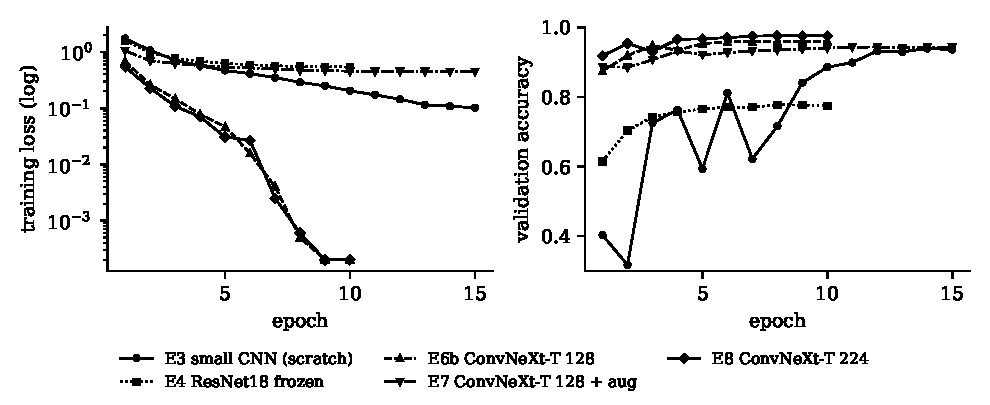
\includegraphics[width=\linewidth]{training_curves.pdf}
\caption{Training loss (log scale) and validation accuracy per epoch for representative runs. The
frozen model (E4) plateaus early; fine-tuned ConvNeXt models drive the training loss to almost zero;
augmentation with label smoothing (E7) keeps the loss high but generalises worse.}
\label{fig:curves}
\end{figure}

%=====================================================================
\section{Step 8 -- Ensembling (E9)}

\paragraph{Idea.} Two good models that see the image at different resolutions should make partly
different mistakes. \textbf{Soft voting} averages the predicted class probabilities of the members
and takes the most probable class.

\paragraph{Result.} E6b (128\,px) + E8 (224\,px): \textbf{0.979} validation, \textbf{0.977} Kaggle
public, i.e.\ $+0.3$ points on both. On validation alone the gain was only 7 images and could have
been noise, but the leaderboard confirmed it independently.

\paragraph{A useful negative finding.} Adding the weaker models to the vote \emph{decreased} accuracy
(E5 + E6b + E8: 0.973; with the small CNN as well: 0.974). Averaging helps only when the members are
comparably strong; a weaker member mostly adds its own errors.

%=====================================================================
\section{Step 9 -- Retraining on all the data (E10a, E10b, E11)}

\paragraph{Idea.} The hyper-parameters were chosen on 80\% of the data. Once a recipe is fixed, the
20\% validation images are just unused training data -- 25\% more examples, most valuable for the small
classes (mozilla has 397 images in total).

\paragraph{A pitfall I fixed first.} With all data in training, the ``validation'' images are part of
the training set, so the code would have reported a meaningless accuracy close to 1.000 and written
it into the Excel sheet. I changed the training script so that full-data runs store no validation
score at all (and added a unit test for it). Without a held-out score, I checked the new submission
files differently: their test predictions agree with the corresponding 80\%-models on 98.2--98.9\% of
the images, and the predicted class distribution matches the training distribution (apple 19.5\%,
mozilla 4.1\%).

\paragraph{Results (Kaggle public only).}
\begin{itemize}[leftmargin=*]
\item E10b = recipe of E8 on 100\%: \textbf{0.978} vs 0.974 for E8 ($+0.43$\pt).
\item E11 = recipe of E9 (ensemble of E10a and E10b): \textbf{0.979} vs 0.977 for E9 ($+0.24$\pt).
\end{itemize}
Both comparisons change only the amount of data, so they measure its effect cleanly.

%=====================================================================
\section{Step 10 -- Error analysis and the resize filter (E12a, E12b, E13)}

\paragraph{Looking at the remaining errors.} E9 makes 41 errors on the 1\,976 validation images. Their
average confidence is 0.79 (correct predictions: 0.98), yet 19 errors have a confidence above 0.9.
\textbf{32 of the 41 errors are 72\,px files}, typically a whatsapp or facebook emoji stored at 72\,px
(rare for these vendors) predicted as apple or google. Visual inspection (Figure~\ref{fig:err}) shows
that many of these designs are almost identical across vendors.

\paragraph{Hypothesis.} A 72\,px image enlarged to 224\,px with \emph{bicubic} interpolation is smoothed:
the exact pixel pattern of the outline (how the vendor anti-aliases its drawing) is blurred.
\emph{Nearest-neighbour} resizing at an integer factor keeps every source pixel intact.

\begin{stepbox}{A clean A/B test at 144\,px (= 2 $\times$ 72)}
E12a: ConvNeXt-Tiny as E6b at 144\,px with bicubic resizing (control). E12b: identical, but
nearest-neighbour resizing. 144\,px keeps each run around 30 minutes.
\end{stepbox}

\begin{table}[H]
\centering\small
\begin{tabular}{lccc}
\toprule
Run & all & 72\,px files (n=1\,178) & 160/240\,px files (n=798) \\
\midrule
E6b  128\,px bicubic & 0.959 & 0.969 & 0.945 \\
E12a 144\,px bicubic & 0.963 & 0.967 & 0.957 \\
E12b 144\,px nearest & \textbf{0.972} & 0.971 & \textbf{0.974} \\
E8   224\,px bicubic & 0.976 & 0.966 & 0.990 \\
E13  216\,px nearest & 0.975 & 0.964 & 0.990 \\
\bottomrule
\end{tabular}
\caption{Validation accuracy split by the original file size.}
\end{table}

\paragraph{What we learned.} Nearest-neighbour gives $+0.9$\pt{} at 144\,px, but -- contrary to my
hypothesis -- mainly on the \emph{large} files (0.957$\to$0.974), not on the 72\,px ones ($+0.4$).
Bicubic \emph{downscaling} from 240 to 144\,px also smears the crisp edge pixels, while
nearest-neighbour keeps them sharp: rendering sharpness is a vendor cue. To see whether this
carries over to high resolution I ran E13 (nearest at 216\,px = 3$\times$72, close to E8's 224\,px):
0.975, the same as E8. At high resolution enough detail survives either way, so the filter no longer
matters. The 72\,px files remain the weak spot of every model (about 0.965--0.97).

\paragraph{Diversity for the ensemble.} Even if E12b and E13 are not better than E8 alone, they look at
the image differently (lower resolution, different filter). The ensemble E8 + E12b + E13 (called E13v)
reaches \textbf{0.981} on validation. Caveat: I compared 11 possible combinations on the same
validation set, and they all lie between 0.977 and 0.981 (a spread of about 8 images), so choosing the
best one carries some selection bias. The full-data version of this ensemble (E14a: E12b recipe on
100\%, E14b: E13 recipe on 100\%, combined with E10b) is \textbf{E15}: \textbf{0.98117} public and
\textbf{0.98238} private, the team's best entry (5th of 18 teams on the private leaderboard). Its
80\%-data counterpart E13v scored 0.97772 public, lower than E11, so on the public half the 3-model
ensemble only paid off after retraining on all data.

%=====================================================================
\section{Step 11 -- Checking for leaks and shortcuts}

The leader scores 0.998, far above our plateau, so I checked whether we were missing an
exploitable property of the data:
\begin{itemize}[leftmargin=*]
\item \textbf{Metadata stacking:} mixing the E1a metadata model's probabilities into the E9
ensemble (weights 0.1--0.5) changes validation accuracy by at most one image (0.9793$\to$0.9798). The
CNNs already capture what the shortcut contained, so ignoring it costs nothing.
\item \textbf{Duplicates:} 297 training images have an exact pixel copy elsewhere in the training set
(none with conflicting labels); 349 test images (3.5\%) are exact copies of training images. Our model
already predicts all 349 correctly -- nothing to gain.
\item \textbf{File IDs:} consecutive training IDs share a label 16.5\% of the time, the same as chance
(16.8\%), so the file order carries no label information.
\end{itemize}

%=====================================================================
\section{Step 12 -- Semi-supervised learning with pseudo-labels (E16)}

\paragraph{Idea.} The 9\,879 unlabelled test images are as many as the training images. Pseudo-labelling
lets the current best model label the test images it is very sure about, and adds them to the training
set.

\paragraph{Choosing the confidence threshold.} The threshold must keep the added labels almost
noise-free. On the validation set, the predictions of the E13v ensemble with confidence $\ge0.99$
cover 91.5\% of the images and are 99.7\% correct. On the test set this threshold selects 9\,046
images. Crucially, the pseudo-labels come from models trained on the 80\% split only, so the
validation set stays untouched and the evaluation remains unbiased.

\paragraph{Setup and result.} E12b recipe (144\,px nearest) + the 9\,046 pseudo-labelled images, single
change. Validation: \textbf{0.977} vs 0.972 (55 $\to$ 45 errors), uniformly on small and large files.
However, inside the 3-model ensemble E16 brings \emph{no} gain (0.981 with or without it).

\paragraph{Interpretation.} The pseudo-labels were produced by that same ensemble, so E16 essentially
learns to imitate the ensemble (self-distillation): the single model catches up with the ensemble but
does not add new knowledge, and the ensemble members become more similar. Pseudo-labelling would be
useful for obtaining a strong \emph{single} model, but it did not move our final score, so it was not
submitted.

%=====================================================================
\section{Submission log and final selection}

\begin{table}[H]
\centering\small
\begin{tabularx}{\linewidth}{lXcc}
\toprule
Submission & What it is & Val acc & Public \\
\midrule
E3   & small CNN, white background (format and protocol check) & 0.936 & 0.936 \\
E8   & ConvNeXt-Tiny 224\,px & 0.976 & 0.974 \\
E9   & ensemble E6b + E8 & 0.979 & 0.977 \\
E10b & E8 recipe on 100\% of the data & n/a & 0.978 \\
E11  & E9 recipe on 100\% of the data & n/a & 0.979 \\
E13v & ensemble E8 + E12b + E13 (80\% data) & 0.981 & 0.978 \\
E15  & E13v recipe on 100\% of the data & n/a & \textbf{0.981} \\
\bottomrule
\end{tabularx}
\caption{All submissions made during this work (7, over two days).}
\end{table}

\paragraph{Final selection (two submissions count).} \textbf{E15} (best public score) and \textbf{E9}
as a hedge. E9 is the only strong model that was measured independently on two different data
sets (our hold-out split and the public leaderboard), whereas the full-data models have only a
public score. If the private half of the test set behaves differently, E9 is the safest fallback.

%=====================================================================
\section{Error analysis of the final models}

\begin{figure}[H]
\centering
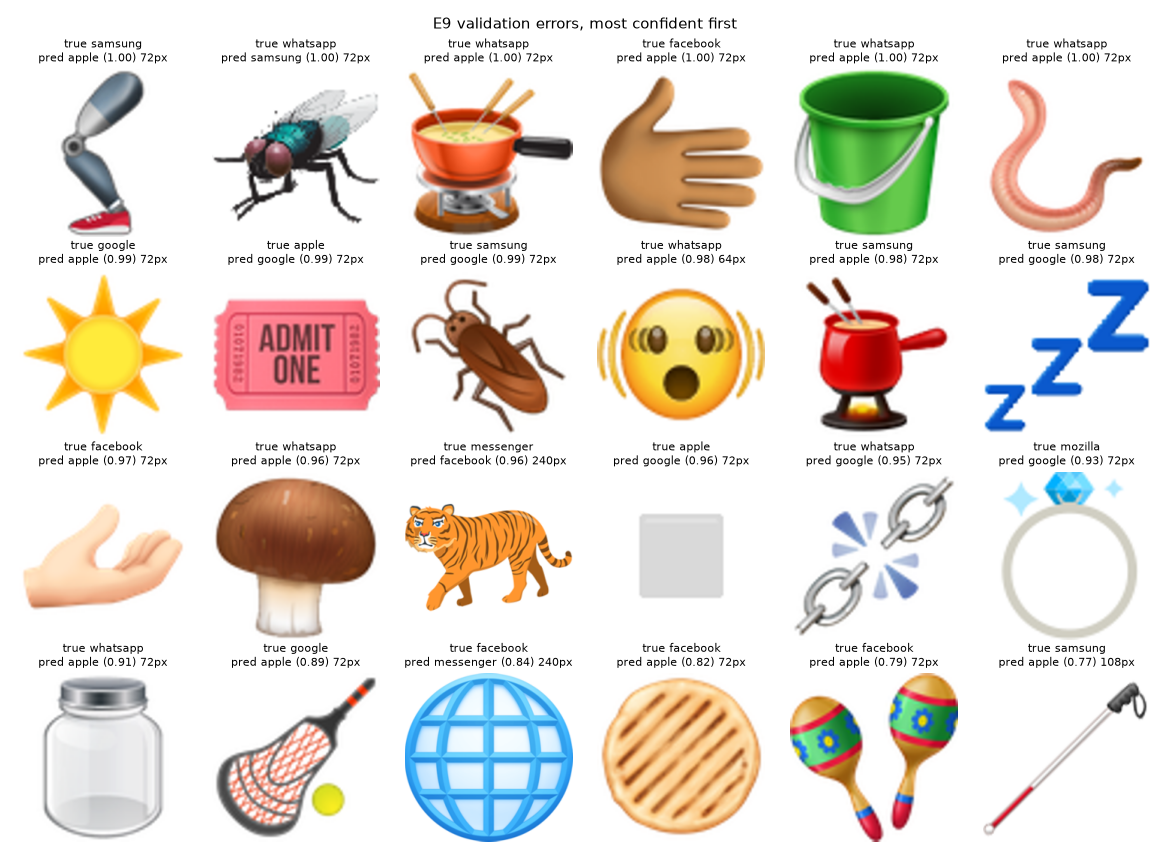
\includegraphics[width=0.82\linewidth]{e9_val_errors.png}
\caption{The 24 most confident validation errors of E9 (true vendor, predicted vendor, confidence,
original file size). Most are 72\,px files whose design is nearly identical across vendors.}
\label{fig:err}
\end{figure}

The most frequent confusions are whatsapp$\to$apple (8), facebook$\to$apple (6), apple$\to$google (5) and
facebook$\to$whatsapp (4). Several of the errors in Figure~\ref{fig:err} (the bucket, the worm, the
fondue pot) look the same as the predicted vendor's version to a human as well. Part of the remaining
2\% error is therefore probably irreducible from the pixels alone.

%=====================================================================
\section{Engineering and reproducibility}

\begin{itemize}[leftmargin=*]
\item \textbf{Code structure} (Python): \code{src/data.py} (loading, the three preprocessing modes
naive / white / rgba, two resize filters, on-disk cache, stratified split), \code{src/classical.py}
(E1a, E1b), \code{src/models.py} (small CNN, \code{timm} backbones, freezing),
\code{src/train.py} (one run: train, evaluate, predict, save), \code{src/ensemble.py} (soft voting),
\code{src/results.py} (JSON record $\to$ Excel), \code{src/submission.py} (writes the CSV and validates
header, 9\,879 unique IDs 10001--19879 and label vocabulary before anything can be uploaded).
\item \textbf{One command per experiment:} \code{run\_experiments.sh} contains the exact command line of
every experiment in this report, e.g.\ \code{./run\_experiments.sh E8}.
\item \textbf{Fixed randomness:} seed 42 for the split, NumPy, PyTorch and the data loader. Training
on Apple MPS is not bit-exact, so a re-run can differ by about 0.2 points.
\item \textbf{Tests:} 15 unit tests (preprocessing, nearest-neighbour behaviour, split, submission
validation, model freezing, Excel export with missing scores).
\item \textbf{Versions} pinned in \code{requirements.txt} (PyTorch 2.14, timm 1.0.30, scikit-learn 1.9).
Every step is a separate git commit with the result in the commit message.
\end{itemize}

%=====================================================================
\section{Limitations and what I would do next}
\begin{itemize}[leftmargin=*]
\item \textbf{Compute-bound choices.} Larger backbones (ConvNeXt-Small/Base), more epochs and several
random seeds per configuration were not tried, because a single 224\,px run takes 1.5--2 hours on the
laptop. A Kaggle GPU notebook would make them feasible and is the most promising next step.
\item \textbf{Single validation split.} The last experiments differ by less than 0.3 points; 5-fold
cross-validation would make these comparisons reliable and remove the selection bias in choosing the
ensemble.
\item \textbf{E7 confounded three changes.} A proper ablation (flip only, affine only, label smoothing
only) would show which part of the augmentation hurt.
\item \textbf{72\,px images} remain the main error source. A model that processes each image at its
native resolution (or a separate model for small files) could address this specifically.
\end{itemize}

\appendix
\section{Complete list of experiments}
\begin{table}[H]
\centering\small
\begin{tabularx}{\linewidth}{llXrr}
\toprule
ID & Model & What changed & Val acc & Kaggle \\
\midrule
E1a & Random forest & metadata only, no pixels (diagnostic) & 0.658 & -- \\
E1b & SVM (RBF) & colour histogram + HOG features, 64\,px & 0.813 & -- \\
E2  & small CNN (scratch) & 3 conv blocks, 96\,px, default RGB conversion & 0.921 & -- \\
E3  & small CNN (scratch) & E2 + alpha composited on white & 0.936 & 0.936 \\
E4  & ResNet18 & ImageNet weights, backbone frozen, 128\,px & 0.775 & -- \\
E5  & ResNet18 & full fine-tuning & 0.937 & -- \\
E6  & EfficientNet-B0 & full fine-tuning & 0.931 & -- \\
E6b & ConvNeXt-Tiny & full fine-tuning, 128\,px & 0.959 & -- \\
E7  & ConvNeXt-Tiny & E6b + flip/rotation/shift + label smoothing & 0.944 & -- \\
E8  & ConvNeXt-Tiny & E6b at 224\,px & 0.976 & 0.974 \\
E9  & ensemble & soft vote E6b + E8 & 0.979 & 0.977 \\
E10a/b & ConvNeXt-Tiny & E6b / E8 retrained on 100\% of the data & n/a & --\,/\,0.978 \\
E11 & ensemble & E10a + E10b (full-data E9) & n/a & 0.979 \\
E12a & ConvNeXt-Tiny & 144\,px, bicubic resize (control) & 0.963 & -- \\
E12b & ConvNeXt-Tiny & 144\,px, nearest-neighbour resize & 0.972 & -- \\
E13 & ConvNeXt-Tiny & 216\,px, nearest-neighbour resize & 0.975 & -- \\
E13v & ensemble & soft vote E8 + E12b + E13 & 0.981 & 0.978 \\
E14a/b, E15 & ensemble & E13v recipe retrained on 100\% of the data & n/a & \textbf{0.981} \\
E16 & ConvNeXt-Tiny & E12b + 9\,046 pseudo-labelled test images & 0.977 & -- \\
\bottomrule
\end{tabularx}
\end{table}

\begin{figure}[H]
\centering
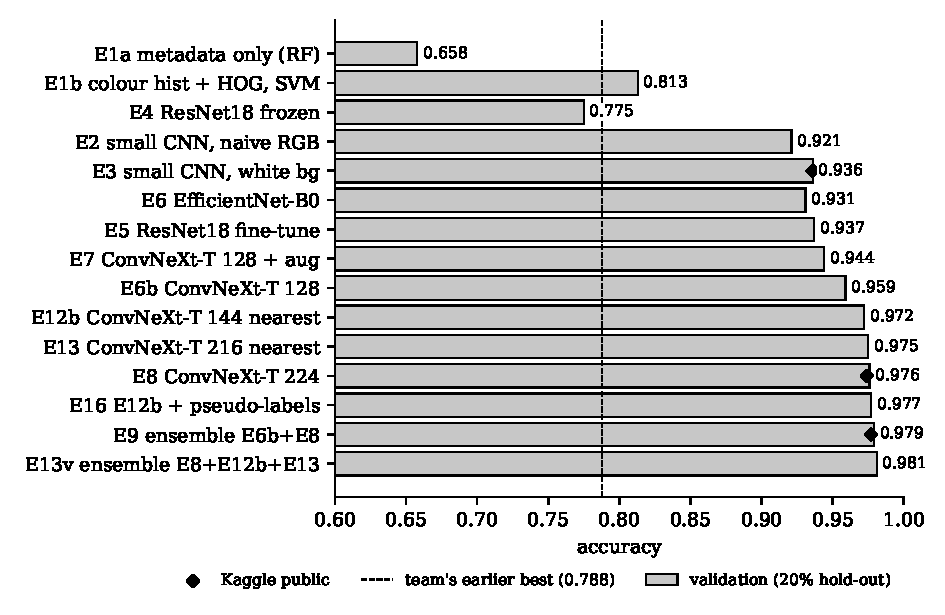
\includegraphics[width=0.9\linewidth]{accuracy_progression.pdf}
\caption{Validation accuracy of the main experiments (bars) and public Kaggle score where submitted (diamonds).}
\end{figure}

\end{document}
